%%%%%%%%%%%%%%%%%%%%%%%%%%%%%%%%%%%%%%%%%%%%%%%%%%%%%%%%%%%%%%%%%%%%%%%%%%%%%%%%
%%%%%%%%%%%%%%%%%%%%%%%%%%%%%%%%%%%%%%%%%%%%%%%%%%%%%%%%%%%%%%%%%%%%%%%%%%%%%%%%
\exercice{Réduction de schéma-bloc~\moyen}
%%%%%%%%%%%%%%%%%%%%%%%%%%%%%%%%%%%%%%%%%%%%%%%%%%%%%%%%%%%%%%%%%%%%%%%%%%%%%%%%
%%%%%%%%%%%%%%%%%%%%%%%%%%%%%%%%%%%%%%%%%%%%%%%%%%%%%%%%%%%%%%%%%%%%%%%%%%%%%%%%

%%%%%%%%%%%%%%%%%%%%%%%%%%%%%%%%%%%%%%%%%%%%%%%%%%%%%%%%%%%%%%%%%%%%%%%%%%%%%%%%
\question{\textbf{Tracer le schéma-bloc dans le cas où l'entrée $P$ 
est nulle. On notera $S_E(p)$ la sortie de ce schéma-bloc.}}
%%%%%%%%%%%%%%%%%%%%%%%%%%%%%%%%%%%%%%%%%%%%%%%%%%%%%%%%%%%%%%%%%%%%%%%%%%%%%%%%
Le schéma-bloc dans le cas pour lequel l'entrée $P$ est nulle est donné 
ci-dessous
%-------------------------------------------------------------------------------
\begin{center}
    \tikzsetnextfilename{ex1-q1-chap_bloc-ext}
    \input{tikz/ex1-q1-chap_bloc.tex}
\end{center}
%-------------------------------------------------------------------------------

%%%%%%%%%%%%%%%%%%%%%%%%%%%%%%%%%%%%%%%%%%%%%%%%%%%%%%%%%%%%%%%%%%%%%%%%%%%%%%%%
\question{\textbf{Déterminer la fonction de transfert $H_E(p)$ 
du schéma-bloc précédent.}}
%%%%%%%%%%%%%%%%%%%%%%%%%%%%%%%%%%%%%%%%%%%%%%%%%%%%%%%%%%%%%%%%%%%%%%%%%%%%%%%%
Pour déterminer la fonction de transfert $H_E(p)$, il nous faut réduire le
schéma-bloc précédent.
%-------------------------------------------------------------------------------
\begin{center}
    \tikzsetnextfilename{ex1-q2-chap_bloc-ext}
    \input{tikz/ex1-q2-chap_bloc.tex}
\end{center}
%-------------------------------------------------------------------------------
On se retrouve avec un boucle de contre réaction unitaire dont la fonction
de transfert est donnée par 
\[
    H_E(p)=\dfrac{KH_1H_2H_3}{1+KH_1H_2H_3}
\]

%%%%%%%%%%%%%%%%%%%%%%%%%%%%%%%%%%%%%%%%%%%%%%%%%%%%%%%%%%%%%%%%%%%%%%%%%%%%%%%%
\question{\textbf{Tracer le schéma-bloc dans le cas où l'entrée $E$ est nulle. 
On notera $S_P(p)$ la sortie de ce schéma-bloc.}}
%%%%%%%%%%%%%%%%%%%%%%%%%%%%%%%%%%%%%%%%%%%%%%%%%%%%%%%%%%%%%%%%%%%%%%%%%%%%%%%%
Le schéma-bloc dans le cas pour lequel l'entrée $E$ est nulle est donné 
ci-dessous
%-------------------------------------------------------------------------------
\begin{center}
    \tikzsetnextfilename{ex1-q3-chap_bloc-ext}
    \begin{tikzpicture}
    \sbEntree{E}
    \sbComp{comp1}{E}
    \sbRelier[$P$]{E}{comp1}
    \sbBlocL{h2}{$H_2$}{comp1}
    \sbRelier{comp1}{h2}
    \sbBlocL{h3}{$H_3$}{h2}
    \sbRelier{h2}{h3}
    \sbSortie[5]{S1}{h3}
    \sbRelier{h3}{S1}
    \sbNomLien[0.8]{S1}{$S_P$}
    \sbDecaleNoeudy[4]{h3}{v}
    \sbBlocr[-1.6]{r2}{$K$}{v}
    \sbBlocr{r3}{$H_1$}{r2}
    \sbRelier{r2}{r3}
    \sbRelieryx{h3-S1}{r2}
    \sbRelierxy{r3}{comp1}
\end{tikzpicture}

\end{center}
%-------------------------------------------------------------------------------

%%%%%%%%%%%%%%%%%%%%%%%%%%%%%%%%%%%%%%%%%%%%%%%%%%%%%%%%%%%%%%%%%%%%%%%%%%%%%%%%
\question{\textbf{Déterminer la fonction de transfert $H_P(p)$ 
du schéma-bloc précédent.}}
%%%%%%%%%%%%%%%%%%%%%%%%%%%%%%%%%%%%%%%%%%%%%%%%%%%%%%%%%%%%%%%%%%%%%%%%%%%%%%%%
Pour déterminer la fonction de transfert $H_E(p)$, il nous faut réduire le
schéma-bloc précédent.
%-------------------------------------------------------------------------------
\begin{center}
    \tikzsetnextfilename{ex1-q4-chap_bloc-ext}
    \begin{tikzpicture}
    \bbr[$P$][ ][$H_2H_3$][][$S_P$][$KH_1$][][ ]
\end{tikzpicture}

\end{center}
%-------------------------------------------------------------------------------
On se retrouve avec un boucle de contre réaction dont la fonction
de transfert est donnée par 
\[
    H_P(p)=\dfrac{H_2H_3}{1+KH_1H_2H_3}
\]

%%%%%%%%%%%%%%%%%%%%%%%%%%%%%%%%%%%%%%%%%%%%%%%%%%%%%%%%%%%%%%%%%%%%%%%%%%%%%%%%
\question{\textbf{Déterminer la sortie globale $S(p)=S_E(p)+S_P(p)$ 
en fonction des entrées $E$, $P$ et des blocs du système.}}
%%%%%%%%%%%%%%%%%%%%%%%%%%%%%%%%%%%%%%%%%%%%%%%%%%%%%%%%%%%%%%%%%%%%%%%%%%%%%%%%
La sortie globale $S(p)$ est alors donnée par la combinaison des deux réponses :

\[
    S(p)=S_E(p)+S_P(p)=H_E(p)E(p) + H_P(p)P(p)
\]
ou encore
\[
    S(p)=\dfrac{KH_1H_2H_3}{1+KH_1H_2H_3}E(p)+\dfrac{H_2H_3}{1+KH_1H_2H_3} P(p)
\]
%%%%%%%%%%%%%%%%%%%%%%%%%%%%%%%%%%%%%%%%%%%%%%%%%%%%%%%%%%%%%%%%%%%%%%%%%%%%%%%%
%%%%%%%%%%%%%%%%%%%%%%%%%%%%%%%%%%%%%%%%%%%%%%%%%%%%%%%%%%%%%%%%%%%%%%%%%%%%%%%%
\exercice{Réduction de schémas fonctionnels~\difficile}
%%%%%%%%%%%%%%%%%%%%%%%%%%%%%%%%%%%%%%%%%%%%%%%%%%%%%%%%%%%%%%%%%%%%%%%%%%%%%%%%
%%%%%%%%%%%%%%%%%%%%%%%%%%%%%%%%%%%%%%%%%%%%%%%%%%%%%%%%%%%%%%%%%%%%%%%%%%%%%%%%
%%%%%%%%%%%%%%%%%%%%%%%%%%%%%%%%%%%%%%%%%%%%%%%%%%%%%%%%%%%%%%%%%%%%%%%%%%%%%%%%
\question{\textbf{Donner la fonction de transfert globale des 
schémas-blocs suivants: (a)}}
%%%%%%%%%%%%%%%%%%%%%%%%%%%%%%%%%%%%%%%%%%%%%%%%%%%%%%%%%%%%%%%%%%%%%%%%%%%%%%%%
%-------------------------------------------------------------------------------
\begin{center} 
    \tikzsetnextfilename{ex2-a1-chap_bloc-ext}
        \begin{tikzpicture}
        \sbEntree{E}
        \sbComp{comp1}{E}
        \sbRelier[$E$]{E}{comp1}
        \sbBloc{h1}{$H_1$}{comp1}
        \sbRelier{comp1}{h1}
        \sbComp{comp2}{h1}
        \sbRelier{h1}{comp2}
        \sbBloc{h2}{$H_2$}{comp2}
        \sbRelier{comp2}{h2}
        \sbBloc{h3}{$H_3$}{h2}
        \sbRelier{h2}{h3}
        \sbBloc{h4}{$H_4$}{h3}
        \sbRelier{h3}{h4}
        \sbSortie[5]{S}{h4}
        \sbRelier{h4}{S}
        \sbNomLien[0.8]{S}{$S$}
        \sbRenvoi[5]{h4-S}{comp1}{}
        \sbRenvoi{h3-h4}{comp2}{}
    \end{tikzpicture}

\end{center}
%-------------------------------------------------------------------------------
Réduisons d'abord la boucle de contre réaction interne :
%-------------------------------------------------------------------------------
\begin{center}
    \tikzsetnextfilename{ex2-a2-chap_bloc-ext}
    \input{tikz/ex2-a2-chap_bloc.tex}
\end{center}
%-------------------------------------------------------------------------------
Réduisons maintenant les blocs en série :
%-------------------------------------------------------------------------------
\begin{center}
    \tikzsetnextfilename{ex2-a3-chap_bloc-ext}
        \begin{tikzpicture}
        \sbEntree{E}
        \sbComp{comp1}{E}
        \sbRelier[$E$]{E}{comp1}
        \sbBloc{br}{$\dfrac{H_1H_2H_3H_4}{1+H_2H_3}$}{comp1}
        \sbRelier{comp1}{br} 
        \sbSortie[5]{S}{br}
        \sbRelier{br}{S}
        \sbNomLien[0.8]{S}{$S$}
        \sbRenvoi[4]{br-S}{comp1}{}
    \end{tikzpicture}

\end{center}
%-------------------------------------------------------------------------------
On obtient après réduction de cette dernière boucle de contre réaction.
%-------------------------------------------------------------------------------
\begin{center}
    \tikzsetnextfilename{ex2-a4-chap_bloc-ext}
        \begin{tikzpicture}
        \sbEntree{E}
        \sbBloc[4]{ke}{$\dfrac{H_1H_2H_3H_4}{1+H_2H_3+H_1H_2H_3H_4}$}{E}
        \sbRelier[$E$]{E}{ke}
        \sbSortie[4]{S}{ke}
        \sbRelier[$S$]{ke}{S}
    \end{tikzpicture}

\end{center}
%-------------------------------------------------------------------------------
%%%%%%%%%%%%%%%%%%%%%%%%%%%%%%%%%%%%%%%%%%%%%%%%%%%%%%%%%%%%%%%%%%%%%%%%%%%%%%%%
\paragraph{(b)}
%%%%%%%%%%%%%%%%%%%%%%%%%%%%%%%%%%%%%%%%%%%%%%%%%%%%%%%%%%%%%%%%%%%%%%%%%%%%%%%%
%-------------------------------------------------------------------------------
\begin{center}
    \tikzsetnextfilename{ex2-b1-chap_bloc-ext}
    \input{tikz/ex2-b1-chap_bloc.tex}
\end{center}
%-------------------------------------------------------------------------------
Déplaçons le point de prélèvement de la boucle de retour inférieur vers 
la droite  :
%-------------------------------------------------------------------------------
\begin{center}
    \tikzsetnextfilename{ex2-b2-chap_bloc-ext}
    \begin{tikzpicture}
    \sbEntree{E}
    \sbComp{a}{E}
    \sbRelier[$E$]{E}{a}
    \sbBloc{b}{$H_1$}{a}
    \sbRelier{a}{b}
    \sbComph{d}{b}
    \sbRelier{b}{d}
    \sbBlocL{f}{$H_2H_3$}{d}
    \sbSortie[5]{S1}{f}
    \sbRelier{f}{S1}
    \sbNomLien[0.8]{S1}{$S$}
    \sbDecaleNoeudy[-4]{f}{u}
    \sbDecaleNoeudy[4]{f}{v}
    \sbBlocr[-1.5]{r1}{$H_4$}{u}
    \sbBlocr{r2}{$\dfrac{H_5}{H_3}$}{v}
    \sbRelieryx{f-S1}{r1}
    \sbRelierxy{r1}{d}
    \sbRelieryx{f-S1}{r2}
    \sbRelierxy{r2}{a}
\end{tikzpicture}

\end{center}
%-------------------------------------------------------------------------------
L'étape précédente nous permet d'identifier une boucle de contre-réaction 
locale. Après réduction de cette boucle, le schéma-blocs dévient :
%-------------------------------------------------------------------------------
\begin{center}
    \tikzsetnextfilename{ex2-b3-chap_bloc-ext}
    \input{tikz/ex2-b3-chap_bloc.tex}
\end{center}
%-------------------------------------------------------------------------------
La réduction de cette dernière boucle de contre-réaction permet d'identifier 
la fonction de transfert globale :
%-------------------------------------------------------------------------------
\begin{center}
    \tikzsetnextfilename{ex2-b4-chap_bloc-ext}
    \input{tikz/ex2-b4-chap_bloc.tex}
\end{center}
%-------------------------------------------------------------------------------
%%%%%%%%%%%%%%%%%%%%%%%%%%%%%%%%%%%%%%%%%%%%%%%%%%%%%%%%%%%%%%%%%%%%%%%%%%%%%%%%
\paragraph{(c)}
%%%%%%%%%%%%%%%%%%%%%%%%%%%%%%%%%%%%%%%%%%%%%%%%%%%%%%%%%%%%%%%%%%%%%%%%%%%%%%%%
%-------------------------------------------------------------------------------
\begin{center}
    \tikzsetnextfilename{ex2-c1-chap_bloc-ext}
        \begin{tikzpicture}
        \sbEntree{E}
        \sbComp{comp1}{E}
        \sbRelier[$E$]{E}{comp1}
        \sbBloc[6]{h1}{$H_1$}{comp1} 
        \sbRelier{comp1}{h1}
        \sbBloc[6]{h2}{$H_2$}{h1}
        \sbRelier{h1}{h2}
        \sbSortie[5]{S}{h2}
        \sbRelier{h2}{S}
        \sbNomLien[0.8]{S}{$S$}
        \sbDecaleNoeudy[3.5]{h1}{u1}
        \sbBlocr[-1.5]{h3}{$H_3$}{u1}
        \sbCompSum[-6]{comp2}{h3}{}{-}{}{+}
        \sbRelier{h3}{comp2}
        \sbRelierxy{comp2}{comp1}
        \sbRelieryx{h1-h2}{h3}
        \sbDecaleNoeudy[3.5]{h3}{u2}
        \sbBlocr[-1.5]{h4}{$H_4$}{u2}
        \sbRelierxy{h4}{comp2}
        \sbRelieryx{h2-S}{h4}
    \end{tikzpicture}

\end{center}
%-------------------------------------------------------------------------------
Déplaçons le point de prélèvement entre les $H_1$ et $H_2$ vers la droite:
%-------------------------------------------------------------------------------
\begin{center}
    \tikzsetnextfilename{ex2-c2-chap_bloc-ext}
    \input{tikz/ex2-c2-chap_bloc.tex}
\end{center}
%-------------------------------------------------------------------------------
On reconnait deux branches en parallèle :
%-------------------------------------------------------------------------------
\begin{center}
    \tikzsetnextfilename{ex2-c3-chap_bloc-ext}
    \input{tikz/ex2-c3-chap_bloc.tex}
\end{center}
%-------------------------------------------------------------------------------
La fonction de transfert globale est donc donné par la réduction de cette 
dernière boucle de contre réaction.
%-------------------------------------------------------------------------------
\begin{center}
    \tikzsetnextfilename{ex2-c4-chap_bloc-ext}
        \begin{tikzpicture}
        \sbEntree{E}
        \sbBloc[4]{ke}{$\dfrac{H_1H_2}{1+H_1H_3H_4-H_1H_2H_4}$}{E}
        \sbRelier[$E$]{E}{ke}
        \sbSortie[4]{S}{ke}
        \sbRelier[$S$]{ke}{S}
    \end{tikzpicture}

\end{center}
%-------------------------------------------------------------------------------
%%%%%%%%%%%%%%%%%%%%%%%%%%%%%%%%%%%%%%%%%%%%%%%%%%%%%%%%%%%%%%%%%%%%%%%%%%%%%%%%
\paragraph{(d)}
%%%%%%%%%%%%%%%%%%%%%%%%%%%%%%%%%%%%%%%%%%%%%%%%%%%%%%%%%%%%%%%%%%%%%%%%%%%%%%%%
%-------------------------------------------------------------------------------
\begin{center}
    \tikzsetnextfilename{ex2-d1-chap_bloc-ext}
    \input{tikz/ex2-d1-chap_bloc.tex}
\end{center}
%-------------------------------------------------------------------------------
Déplaçons vers la droite le point de prélèvement situé entre les 
blocs $H_3$ et $H_4$:
%-------------------------------------------------------------------------------
\begin{center}
    \tikzsetnextfilename{ex2-d2-chap_bloc-ext}
    \input{tikz/ex2-d2-chap_bloc.tex}
\end{center}
%-------------------------------------------------------------------------------
Réduisons la boucle de contre-réaction et les blocs en parallèle.
%-------------------------------------------------------------------------------
\begin{center}
    \tikzsetnextfilename{ex2-d3-chap_bloc-ext}
    \begin{tikzpicture}
    \sbEntree{E}
    \sbComp{comp1}{E}
    \sbRelier[$E$]{E}{comp1}
    \sbBloc{h1}{$H_1$}{comp1}
    \sbRelier{comp1}{h1}
    \sbComp{comp2}{h1}
    \sbRelier{h1}{comp2}
    \sbBlocL{h2}{$H_2$}{comp2}
    \sbBlocL{h4}{$\dfrac{H_3H_4}{1+H_3H_4G_4}$}{h2}
    \sbSortie[5]{S}{h4}
    \sbRelier{h4}{S}
    \sbNomLien[0.8]{S}{$S$}
    \sbDecaleNoeudy{h4}{v}
    \sbBlocr[4]{g3}{$\dfrac{G_3}{H_4}$}{v}
    \sbRelieryx{h4-S}{g3}
    \sbRelierxy{g3}{comp2}
    \sbDecaleNoeudy[9]{h4}{w}
    \sbBlocr[4]{g2}{$\dfrac{G_2-G_1H_4}{H_4}$}{w}
    \sbRelierxy{g2}{comp1}
    \sbRelieryx{h4-S}{g2}
\end{tikzpicture}

\end{center}
%-------------------------------------------------------------------------------
Réduisons la nouvelle boucle de contre-réaction interne :
%-------------------------------------------------------------------------------
\begin{center}
    \tikzsetnextfilename{ex2-d4-chap_bloc-ext}
    \input{tikz/ex2-d4-chap_bloc.tex}
\end{center}
%-------------------------------------------------------------------------------
Cette dernière boucle peut être réduite pour obtenir la fonction de 
transfert globale :
%-------------------------------------------------------------------------------
\begin{center}
    \tikzsetnextfilename{ex2-d5-chap_bloc-ext}
    \input{tikz/ex2-d5-chap_bloc.tex}
\end{center}
%-------------------------------------------------------------------------------
\clearpage
%%%%%%%%%%%%%%%%%%%%%%%%%%%%%%%%%%%%%%%%%%%%%%%%%%%%%%%%%%%%%%%%%%%%%%%%%%%%%%%%
%%%%%%%%%%%%%%%%%%%%%%%%%%%%%%%%%%%%%%%%%%%%%%%%%%%%%%%%%%%%%%%%%%%%%%%%%%%%%%%%
\exercice{Graphe de fluence~\difficile}
%%%%%%%%%%%%%%%%%%%%%%%%%%%%%%%%%%%%%%%%%%%%%%%%%%%%%%%%%%%%%%%%%%%%%%%%%%%%%%%%
%%%%%%%%%%%%%%%%%%%%%%%%%%%%%%%%%%%%%%%%%%%%%%%%%%%%%%%%%%%%%%%%%%%%%%%%%%%%%%%%
%%%%%%%%%%%%%%%%%%%%%%%%%%%%%%%%%%%%%%%%%%%%%%%%%%%%%%%%%%%%%%%%%%%%%%%%%%%%%%%%
\question{\textbf{Donner les relations du modèle dans le domaine de Laplace}}
%%%%%%%%%%%%%%%%%%%%%%%%%%%%%%%%%%%%%%%%%%%%%%%%%%%%%%%%%%%%%%%%%%%%%%%%%%%%%%%%
Dans le domaine de Laplace, ces dernières deviennent :
%-------------------------------------------------------------------------------
\begin{align*}
    I_1(p)=\dfrac{1}{R_1}\big(V_1(p)-V_2(p)\big)\\
    I_2(p)=I_1(p)-\dfrac{1}{R_2}V_2(p)
\end{align*}
%-------------------------------------------------------------------------------
Notons que la tension $V_2(p)$ est donnée par :
\[
    V_2(p)=\dfrac{1}{Cp}I_2(p)
\]
%%%%%%%%%%%%%%%%%%%%%%%%%%%%%%%%%%%%%%%%%%%%%%%%%%%%%%%%%%%%%%%%%%%%%%%%%%%%%%%%
\question{\textbf{Tracer le graphe de fluence de ce modèle.}}
%%%%%%%%%%%%%%%%%%%%%%%%%%%%%%%%%%%%%%%%%%%%%%%%%%%%%%%%%%%%%%%%%%%%%%%%%%%%%%%%
%-------------------------------------------------------------------------------
\begin{center}
    \tikzsetnextfilename{gf_exo3_2-chap-bloc-ext}
    \begin{tikzpicture}
    \gfEntree{$V_1$}{E}
    \gfNoeud[5]{$I_1$}{E}{I1}
    \gfNoeud[5]{$I_2$}[-]{I1}{I2}
    \gfSortie[5]{$V_2$}{I2}{S}
    \gfRelier[$\dfrac{1}{R_1}$][][1.6]{E}{I1}
    \gfRelier[1]{I1}{I2}
    \gfRelier[$\dfrac{1}{Cp}$][-][1.6]{I2}{S}
    \gfRelierB[-$\dfrac{1}{R_1}$][-][-0.5][0]{S}{I1}
    \gfRelierB[-$\dfrac{1}{R_2}$][+][0][1.0]{S}{I2}
\end{tikzpicture}

\end{center}
%-------------------------------------------------------------------------------
%%%%%%%%%%%%%%%%%%%%%%%%%%%%%%%%%%%%%%%%%%%%%%%%%%%%%%%%%%%%%%%%%%%%%%%%%%%%%%%%
\question{\textbf{À partir de ce graphe et appliquant la règle de Mason, 
déterminer la fonction de transfert global de ce système.}}
%%%%%%%%%%%%%%%%%%%%%%%%%%%%%%%%%%%%%%%%%%%%%%%%%%%%%%%%%%%%%%%%%%%%%%%%%%%%%%%%
Le graphe de fluence présente deux boucles disjointes :
%-------------------------------------------------------------------------------
\begin{itemize}
    \item $\{I_1\rightarrow I_2\rightarrow V_2\rightarrow I_1\}$ 
          de gain $B_1=-\dfrac{1}{R_1Cp}$ 
    \item $\{I_2\rightarrow V_2\}$ de gain $B_2=-\dfrac{1}{R_2Cp}$ 
\end{itemize}
%-------------------------------------------------------------------------------
Le déterminant du graphe est donc donné par :
\[
    \Delta=1-B_1-B_2=\dfrac{R_1R_2C^2p^2+R_2Cp+R_1Cp}{R_1R_2C^2p^2}
\]

Le graphe ne présente qu'un parcours ouvert :
\[
    \{V_1\rightarrow I_1\rightarrow I_2\rightarrow V_2\}
\]
de gain $G_1=\dfrac{1}{R_1Cp}$ et de déterminant $\Delta_1=1$

D'après la règle de Mason, la transmitance est alors donnée par :
\[
    H(p)=\dfrac{V_2(p)}{V_1(p)}=\dfrac{R_2}{R_1R_2Cp+ R_1+R_2}
\]
\clearpage
%%%%%%%%%%%%%%%%%%%%%%%%%%%%%%%%%%%%%%%%%%%%%%%%%%%%%%%%%%%%%%%%%%%%%%%%%%%%%%%%
%%%%%%%%%%%%%%%%%%%%%%%%%%%%%%%%%%%%%%%%%%%%%%%%%%%%%%%%%%%%%%%%%%%%%%%%%%%%%%%%
\exercice{Schéma-blocs dans le domaine temporel~\moyen}
%%%%%%%%%%%%%%%%%%%%%%%%%%%%%%%%%%%%%%%%%%%%%%%%%%%%%%%%%%%%%%%%%%%%%%%%%%%%%%%%
%%%%%%%%%%%%%%%%%%%%%%%%%%%%%%%%%%%%%%%%%%%%%%%%%%%%%%%%%%%%%%%%%%%%%%%%%%%%%%%%
%%%%%%%%%%%%%%%%%%%%%%%%%%%%%%%%%%%%%%%%%%%%%%%%%%%%%%%%%%%%%%%%%%%%%%%%%%%%%%%%
\question{\textbf{Tracer le schéma-bloc dans le domaine temporel de l'équation 
différentielle suivante:}}
%%%%%%%%%%%%%%%%%%%%%%%%%%%%%%%%%%%%%%%%%%%%%%%%%%%%%%%%%%%%%%%%%%%%%%%%%%%%%%%%
\[
    \dot{s}(t)=a\big(e(t)+s(t)\big)
\]
%-------------------------------------------------------------------------------
\begin{center}
    \tikzsetnextfilename{sbdt_eqdiff1-chap_bloc-ext}
    \begin{tikzpicture}
    \sbEntree{E1}
    \sbCompSum[5.0]{comp}{E1}{}{+}{+}{}
    \sbRelier[$e(t)$]{E1}{comp}
    \sbBlocT[3]{T}{comp}
    \sbRelier[]{comp}{T}
    \sbInt[3]{B1}{T}
    \sbRelier[$\dot{s}(t)$]{T}{B1}
    \sbSortie[6]{S1}{B1}
    \sbRelier[$s(t)$]{B1}{S1}
    \sbRenvoi[5]{B1-S1}{comp}{}
\end{tikzpicture}


\end{center}
%-------------------------------------------------------------------------------
%%%%%%%%%%%%%%%%%%%%%%%%%%%%%%%%%%%%%%%%%%%%%%%%%%%%%%%%%%%%%%%%%%%%%%%%%%%%%%%%
\question{\textbf{Réduiser le schéma-bloc sous une forme faisant apparaitre 
l'opérateur intégral}}
%%%%%%%%%%%%%%%%%%%%%%%%%%%%%%%%%%%%%%%%%%%%%%%%%%%%%%%%%%%%%%%%%%%%%%%%%%%%%%%%
Sous forme d'opérateur, on réduira ce schéma-bloc par 
la relation suivante :
\[
    S=a\mathcal{I}\big(E+S\big)
\]
%%%%%%%%%%%%%%%%%%%%%%%%%%%%%%%%%%%%%%%%%%%%%%%%%%%%%%%%%%%%%%%%%%%%%%%%%%%%%%%%
\question{\textbf{Donner le rapport de l'entrée sur la sortie}}
%%%%%%%%%%%%%%%%%%%%%%%%%%%%%%%%%%%%%%%%%%%%%%%%%%%%%%%%%%%%%%%%%%%%%%%%%%%%%%%%
Le rapport de la sortie sur l'entrée
\[
    \dfrac{S}{E}=\dfrac{a\mathcal{I}}{1-a\mathcal{I}}
\]
%%%%%%%%%%%%%%%%%%%%%%%%%%%%%%%%%%%%%%%%%%%%%%%%%%%%%%%%%%%%%%%%%%%%%%%%%%%%%%%%
%%%%%%%%%%%%%%%%%%%%%%%%%%%%%%%%%%%%%%%%%%%%%%%%%%%%%%%%%%%%%%%%%%%%%%%%%%%%%%%%
\exercice{Schéma-blocs dans le domaine temporel (2)~\moyen}
%%%%%%%%%%%%%%%%%%%%%%%%%%%%%%%%%%%%%%%%%%%%%%%%%%%%%%%%%%%%%%%%%%%%%%%%%%%%%%%%
%%%%%%%%%%%%%%%%%%%%%%%%%%%%%%%%%%%%%%%%%%%%%%%%%%%%%%%%%%%%%%%%%%%%%%%%%%%%%%%%
%%%%%%%%%%%%%%%%%%%%%%%%%%%%%%%%%%%%%%%%%%%%%%%%%%%%%%%%%%%%%%%%%%%%%%%%%%%%%%%%
\question{\textbf{Tracer le schéma-bloc dans le domaine temporel de l'équation 
différentielle suivante:}}
%%%%%%%%%%%%%%%%%%%%%%%%%%%%%%%%%%%%%%%%%%%%%%%%%%%%%%%%%%%%%%%%%%%%%%%%%%%%%%%%
\[
    \dot{s}(t)=\dot{e}(t)+as(t)
\]
Il est plus d'intégrer l'équation différentielle avant de la réprésenter
graphiquement. Ainsi, elle devient :
\[
    s(t)=e(t)+a\int_{-\infty}^t s(\tau) \dd{\tau}
\]
%-------------------------------------------------------------------------------
\begin{center}
    \tikzsetnextfilename{sbdt_eqdiff3-chap_bloc-ext}
    \begin{tikzpicture}
    \sbEntree{E1}
    \sbCompSum[5.0]{comp}{E1}{}{+}{+}{}
    \sbRelier[$x(t)$]{E1}{comp}
    \sbSortie[12]{S1}{comp}
    \node [left of =S1, node distance=4em] (ref) {};
    \sbRelierNoDraw[]{ref}{S1}
    \sbRelier[$y(t)$]{comp}{S1}
    \sbDecaleNoeudy{S1}{R}
    \sbIntr[4]{B1}{R}
    \sbRelieryx{ref-S1}{B1}
    \sbBlocTr[2.5]{R1}{B1}
    \sbRelier[]{B1}{R1}
    \sbRelierxy[]{R1}{comp}
\end{tikzpicture}


\end{center}
%-------------------------------------------------------------------------------
%%%%%%%%%%%%%%%%%%%%%%%%%%%%%%%%%%%%%%%%%%%%%%%%%%%%%%%%%%%%%%%%%%%%%%%%%%%%%%%%
\question{\textbf{Réduiser le schéma-bloc sous une forme faisant apparaitre 
l'opérateur intégral}}
%%%%%%%%%%%%%%%%%%%%%%%%%%%%%%%%%%%%%%%%%%%%%%%%%%%%%%%%%%%%%%%%%%%%%%%%%%%%%%%%
Sous forme d'opérateur, on réduira ce schéma-bloc par 
la relation suivante :
\[
    S=E+a\mathcal{I}S
\]
%%%%%%%%%%%%%%%%%%%%%%%%%%%%%%%%%%%%%%%%%%%%%%%%%%%%%%%%%%%%%%%%%%%%%%%%%%%%%%%%
\question{\textbf{Donner le rapport de l'entrée sur la sortie}}
%%%%%%%%%%%%%%%%%%%%%%%%%%%%%%%%%%%%%%%%%%%%%%%%%%%%%%%%%%%%%%%%%%%%%%%%%%%%%%%%
Le rapport de la sortie sur l'entrée
\[
    \dfrac{S}{E}=\dfrac{1}{1-a\mathcal{I}}
\]
